% Created by tikzDevice version 0.10.1 on 2016-08-19 16:15:04
% !TEX encoding = UTF-8 Unicode
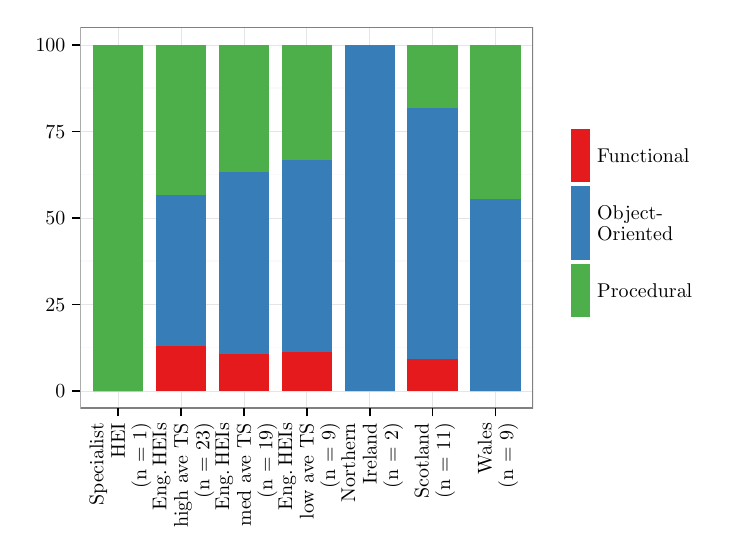
\begin{tikzpicture}[x=1pt,y=1pt]
\definecolor{fillColor}{RGB}{255,255,255}
\path[use as bounding box,fill=fillColor,fill opacity=0.00] (0,0) rectangle (252.94,180.67);
\begin{scope}
\path[clip] (  0.00,  0.00) rectangle (252.94,180.67);
\definecolor{drawColor}{RGB}{255,255,255}
\definecolor{fillColor}{RGB}{255,255,255}

\path[draw=drawColor,line width= 0.6pt,line join=round,line cap=round,fill=fillColor] (  0.00,  0.00) rectangle (252.94,180.68);
\end{scope}
\begin{scope}
\path[clip] ( 19.04, 43.19) rectangle (182.66,180.67);
\definecolor{fillColor}{RGB}{255,255,255}

\path[fill=fillColor] ( 19.04, 43.19) rectangle (182.66,180.67);
\definecolor{drawColor}{gray}{0.98}

\path[draw=drawColor,line width= 0.6pt,line join=round] ( 19.04, 65.06) --
	(182.66, 65.06);

\path[draw=drawColor,line width= 0.6pt,line join=round] ( 19.04, 96.31) --
	(182.66, 96.31);

\path[draw=drawColor,line width= 0.6pt,line join=round] ( 19.04,127.56) --
	(182.66,127.56);

\path[draw=drawColor,line width= 0.6pt,line join=round] ( 19.04,158.80) --
	(182.66,158.80);
\definecolor{drawColor}{gray}{0.90}

\path[draw=drawColor,line width= 0.2pt,line join=round] ( 19.04, 49.44) --
	(182.66, 49.44);

\path[draw=drawColor,line width= 0.2pt,line join=round] ( 19.04, 80.69) --
	(182.66, 80.69);

\path[draw=drawColor,line width= 0.2pt,line join=round] ( 19.04,111.93) --
	(182.66,111.93);

\path[draw=drawColor,line width= 0.2pt,line join=round] ( 19.04,143.18) --
	(182.66,143.18);

\path[draw=drawColor,line width= 0.2pt,line join=round] ( 19.04,174.43) --
	(182.66,174.43);

\path[draw=drawColor,line width= 0.2pt,line join=round] ( 32.68, 43.19) --
	( 32.68,180.67);

\path[draw=drawColor,line width= 0.2pt,line join=round] ( 55.40, 43.19) --
	( 55.40,180.67);

\path[draw=drawColor,line width= 0.2pt,line join=round] ( 78.13, 43.19) --
	( 78.13,180.67);

\path[draw=drawColor,line width= 0.2pt,line join=round] (100.85, 43.19) --
	(100.85,180.67);

\path[draw=drawColor,line width= 0.2pt,line join=round] (123.58, 43.19) --
	(123.58,180.67);

\path[draw=drawColor,line width= 0.2pt,line join=round] (146.30, 43.19) --
	(146.30,180.67);

\path[draw=drawColor,line width= 0.2pt,line join=round] (169.03, 43.19) --
	(169.03,180.67);
\definecolor{fillColor}{RGB}{228,26,28}

\path[fill=fillColor] ( 23.59, 49.44) rectangle ( 41.77, 49.44);
\definecolor{fillColor}{RGB}{55,126,184}

\path[fill=fillColor] ( 23.59, 49.44) rectangle ( 41.77, 49.44);
\definecolor{fillColor}{RGB}{77,175,74}

\path[fill=fillColor] ( 23.59, 49.44) rectangle ( 41.77,174.43);
\definecolor{fillColor}{RGB}{228,26,28}

\path[fill=fillColor] ( 46.31, 49.44) rectangle ( 64.49, 65.74);
\definecolor{fillColor}{RGB}{55,126,184}

\path[fill=fillColor] ( 46.31, 65.74) rectangle ( 64.49,120.08);
\definecolor{fillColor}{RGB}{77,175,74}

\path[fill=fillColor] ( 46.31,120.08) rectangle ( 64.49,174.43);
\definecolor{fillColor}{RGB}{228,26,28}

\path[fill=fillColor] ( 69.04, 49.44) rectangle ( 87.22, 62.60);
\definecolor{fillColor}{RGB}{55,126,184}

\path[fill=fillColor] ( 69.04, 62.60) rectangle ( 87.22,128.38);
\definecolor{fillColor}{RGB}{77,175,74}

\path[fill=fillColor] ( 69.04,128.38) rectangle ( 87.22,174.43);
\definecolor{fillColor}{RGB}{228,26,28}

\path[fill=fillColor] ( 91.76, 49.44) rectangle (109.94, 63.33);
\definecolor{fillColor}{RGB}{55,126,184}

\path[fill=fillColor] ( 91.76, 63.33) rectangle (109.94,132.76);
\definecolor{fillColor}{RGB}{77,175,74}

\path[fill=fillColor] ( 91.76,132.76) rectangle (109.94,174.43);
\definecolor{fillColor}{RGB}{228,26,28}

\path[fill=fillColor] (114.49, 49.44) rectangle (132.67, 49.44);
\definecolor{fillColor}{RGB}{55,126,184}

\path[fill=fillColor] (114.49, 49.44) rectangle (132.67,174.43);
\definecolor{fillColor}{RGB}{77,175,74}

\path[fill=fillColor] (114.49,174.43) rectangle (132.67,174.43);
\definecolor{fillColor}{RGB}{228,26,28}

\path[fill=fillColor] (137.21, 49.44) rectangle (155.39, 60.80);
\definecolor{fillColor}{RGB}{55,126,184}

\path[fill=fillColor] (137.21, 60.80) rectangle (155.39,151.70);
\definecolor{fillColor}{RGB}{77,175,74}

\path[fill=fillColor] (137.21,151.70) rectangle (155.39,174.43);
\definecolor{fillColor}{RGB}{228,26,28}

\path[fill=fillColor] (159.94, 49.44) rectangle (178.12, 49.44);
\definecolor{fillColor}{RGB}{55,126,184}

\path[fill=fillColor] (159.94, 49.44) rectangle (178.12,118.88);
\definecolor{fillColor}{RGB}{77,175,74}

\path[fill=fillColor] (159.94,118.88) rectangle (178.12,174.43);
\definecolor{drawColor}{gray}{0.50}

\path[draw=drawColor,line width= 0.6pt,line join=round,line cap=round] ( 19.04, 43.19) rectangle (182.66,180.67);
\end{scope}
\begin{scope}
\path[clip] (  0.00,  0.00) rectangle (252.94,180.67);
\definecolor{drawColor}{RGB}{0,0,0}

\node[text=drawColor,anchor=base east,inner sep=0pt, outer sep=0pt, scale=  0.72] at ( 13.64, 46.96) {0};

\node[text=drawColor,anchor=base east,inner sep=0pt, outer sep=0pt, scale=  0.72] at ( 13.64, 78.21) {25};

\node[text=drawColor,anchor=base east,inner sep=0pt, outer sep=0pt, scale=  0.72] at ( 13.64,109.45) {50};

\node[text=drawColor,anchor=base east,inner sep=0pt, outer sep=0pt, scale=  0.72] at ( 13.64,140.70) {75};

\node[text=drawColor,anchor=base east,inner sep=0pt, outer sep=0pt, scale=  0.72] at ( 13.64,171.95) {100};
\end{scope}
\begin{scope}
\path[clip] (  0.00,  0.00) rectangle (252.94,180.67);
\definecolor{drawColor}{RGB}{0,0,0}

\path[draw=drawColor,line width= 0.6pt,line join=round] ( 16.04, 49.44) --
	( 19.04, 49.44);

\path[draw=drawColor,line width= 0.6pt,line join=round] ( 16.04, 80.69) --
	( 19.04, 80.69);

\path[draw=drawColor,line width= 0.6pt,line join=round] ( 16.04,111.93) --
	( 19.04,111.93);

\path[draw=drawColor,line width= 0.6pt,line join=round] ( 16.04,143.18) --
	( 19.04,143.18);

\path[draw=drawColor,line width= 0.6pt,line join=round] ( 16.04,174.43) --
	( 19.04,174.43);
\end{scope}
\begin{scope}
\path[clip] (  0.00,  0.00) rectangle (252.94,180.67);
\definecolor{drawColor}{RGB}{0,0,0}

\path[draw=drawColor,line width= 0.6pt,line join=round] ( 32.68, 40.19) --
	( 32.68, 43.19);

\path[draw=drawColor,line width= 0.6pt,line join=round] ( 55.40, 40.19) --
	( 55.40, 43.19);

\path[draw=drawColor,line width= 0.6pt,line join=round] ( 78.13, 40.19) --
	( 78.13, 43.19);

\path[draw=drawColor,line width= 0.6pt,line join=round] (100.85, 40.19) --
	(100.85, 43.19);

\path[draw=drawColor,line width= 0.6pt,line join=round] (123.58, 40.19) --
	(123.58, 43.19);

\path[draw=drawColor,line width= 0.6pt,line join=round] (146.30, 40.19) --
	(146.30, 43.19);

\path[draw=drawColor,line width= 0.6pt,line join=round] (169.03, 40.19) --
	(169.03, 43.19);
\end{scope}
\begin{scope}
\path[clip] (  0.00,  0.00) rectangle (252.94,180.67);
\definecolor{drawColor}{RGB}{0,0,0}

\node[text=drawColor,rotate= 90.00,anchor=base east,inner sep=0pt, outer sep=0pt, scale=  0.72] at ( 27.38, 37.79) {Specialist};

\node[text=drawColor,rotate= 90.00,anchor=base east,inner sep=0pt, outer sep=0pt, scale=  0.72] at ( 35.16, 37.79) {HEI};

\node[text=drawColor,rotate= 90.00,anchor=base east,inner sep=0pt, outer sep=0pt, scale=  0.72] at ( 42.93, 37.79) {(n = 1)};

\node[text=drawColor,rotate= 90.00,anchor=base east,inner sep=0pt, outer sep=0pt, scale=  0.72] at ( 50.11, 37.79) {Eng.\,HEIs};

\node[text=drawColor,rotate= 90.00,anchor=base east,inner sep=0pt, outer sep=0pt, scale=  0.72] at ( 57.88, 37.79) {high ave TS};

\node[text=drawColor,rotate= 90.00,anchor=base east,inner sep=0pt, outer sep=0pt, scale=  0.72] at ( 65.66, 37.79) {(n = 23)};

\node[text=drawColor,rotate= 90.00,anchor=base east,inner sep=0pt, outer sep=0pt, scale=  0.72] at ( 72.83, 37.79) {Eng.\,HEIs};

\node[text=drawColor,rotate= 90.00,anchor=base east,inner sep=0pt, outer sep=0pt, scale=  0.72] at ( 80.61, 37.79) {med ave TS};

\node[text=drawColor,rotate= 90.00,anchor=base east,inner sep=0pt, outer sep=0pt, scale=  0.72] at ( 88.38, 37.79) {(n = 19)};

\node[text=drawColor,rotate= 90.00,anchor=base east,inner sep=0pt, outer sep=0pt, scale=  0.72] at ( 95.56, 37.79) {Eng.\,HEIs};

\node[text=drawColor,rotate= 90.00,anchor=base east,inner sep=0pt, outer sep=0pt, scale=  0.72] at (103.33, 37.79) {low ave TS};

\node[text=drawColor,rotate= 90.00,anchor=base east,inner sep=0pt, outer sep=0pt, scale=  0.72] at (111.11, 37.79) {(n = 9)};

\node[text=drawColor,rotate= 90.00,anchor=base east,inner sep=0pt, outer sep=0pt, scale=  0.72] at (118.28, 37.79) {Northern};

\node[text=drawColor,rotate= 90.00,anchor=base east,inner sep=0pt, outer sep=0pt, scale=  0.72] at (126.06, 37.79) {Ireland};

\node[text=drawColor,rotate= 90.00,anchor=base east,inner sep=0pt, outer sep=0pt, scale=  0.72] at (133.83, 37.79) {(n = 2)};

\node[text=drawColor,rotate= 90.00,anchor=base east,inner sep=0pt, outer sep=0pt, scale=  0.72] at (144.89, 37.79) {Scotland};

\node[text=drawColor,rotate= 90.00,anchor=base east,inner sep=0pt, outer sep=0pt, scale=  0.72] at (152.67, 37.79) {(n = 11)};

\node[text=drawColor,rotate= 90.00,anchor=base east,inner sep=0pt, outer sep=0pt, scale=  0.72] at (167.62, 37.79) {Wales};

\node[text=drawColor,rotate= 90.00,anchor=base east,inner sep=0pt, outer sep=0pt, scale=  0.72] at (175.40, 37.79) {(n = 9)};
\end{scope}
\begin{scope}
\path[clip] (  0.00,  0.00) rectangle (252.94,180.67);
\definecolor{fillColor}{RGB}{255,255,255}

\path[fill=fillColor] (191.20, 71.20) rectangle (244.41,152.66);
\end{scope}
\begin{scope}
\path[clip] (  0.00,  0.00) rectangle (252.94,180.67);
\definecolor{fillColor}{RGB}{228,26,28}

\path[fill=fillColor] (196.18,124.98) rectangle (203.29,144.07);
\end{scope}
\begin{scope}
\path[clip] (  0.00,  0.00) rectangle (252.94,180.67);
\definecolor{fillColor}{RGB}{55,126,184}

\path[fill=fillColor] (196.18, 96.69) rectangle (203.29,123.56);
\end{scope}
\begin{scope}
\path[clip] (  0.00,  0.00) rectangle (252.94,180.67);
\definecolor{fillColor}{RGB}{77,175,74}

\path[fill=fillColor] (196.18, 76.18) rectangle (203.29, 95.27);
\end{scope}
\begin{scope}
\path[clip] (  0.00,  0.00) rectangle (252.94,180.67);
\definecolor{drawColor}{RGB}{0,0,0}

\node[text=drawColor,anchor=base west,inner sep=0pt, outer sep=0pt, scale=  0.72] at (205.81,139.82) {};

\node[text=drawColor,anchor=base west,inner sep=0pt, outer sep=0pt, scale=  0.72] at (205.81,132.05) {Functional};

\node[text=drawColor,anchor=base west,inner sep=0pt, outer sep=0pt, scale=  0.72] at (205.81,124.27) {};
\end{scope}
\begin{scope}
\path[clip] (  0.00,  0.00) rectangle (252.94,180.67);
\definecolor{drawColor}{RGB}{0,0,0}

\node[text=drawColor,anchor=base west,inner sep=0pt, outer sep=0pt, scale=  0.72] at (205.81,119.31) {};

\node[text=drawColor,anchor=base west,inner sep=0pt, outer sep=0pt, scale=  0.72] at (205.81,111.53) {Object-};

\node[text=drawColor,anchor=base west,inner sep=0pt, outer sep=0pt, scale=  0.72] at (205.81,103.76) {Oriented};

\node[text=drawColor,anchor=base west,inner sep=0pt, outer sep=0pt, scale=  0.72] at (205.81, 95.98) {};
\end{scope}
\begin{scope}
\path[clip] (  0.00,  0.00) rectangle (252.94,180.67);
\definecolor{drawColor}{RGB}{0,0,0}

\node[text=drawColor,anchor=base west,inner sep=0pt, outer sep=0pt, scale=  0.72] at (205.81, 91.02) {};

\node[text=drawColor,anchor=base west,inner sep=0pt, outer sep=0pt, scale=  0.72] at (205.81, 83.25) {Procedural};

\node[text=drawColor,anchor=base west,inner sep=0pt, outer sep=0pt, scale=  0.72] at (205.81, 75.47) {};
\end{scope}
\end{tikzpicture}
